Though testing for different variables, certain wind farm attributes were common to all case studies.
A brief list of these common variables is described below.

\subsubsection{Wind Turbine Specifications} \label{sec:turb}
	We used IEA 5 MW offshore reference turbine in cs3 \& cs4, since our wind farms are modelled after an offshore location.
	The this turbine is open source, and the turbine is designed as baseline for offshore wind turbine specifications \cite{NREL5MW}.
	The power curve for the IEA 5 MW turbine is defined as shown in \cref{eq:power,fig:5MW}.
	The specifications of the turbine necessary for our simplified version of Bastankhah's Gaussian wake model (used in cs3) are shown in \cref{tab:turb-att}.  %
	\begin{equation}\label{eq:power}
		P(V) = 
		\begin{cases} 
			0 & V < V_{\textit{cut-in}} \\
			P_{\textit{rated}}\bigg(\frac{V-V_{\textit{cut-in}}}{V_{\textit{rated}}-V_{\textit{cut-in}}}\bigg)^3 & V_{\textit{cut-in}}\leq V < V_{\textit{rated}} \\
			P_{\textit{rated}} & V_{\textit{rated}} \leq V < V_{\textit{cut-out}} \\
			0 & V \geq V_{\textit{cut-out}}
		\end{cases}
	\end{equation}
	%
	\begin{figure}[H]
	    \centering
	   % \includegraphics[width=2.6in]{./figures/iea37-5mw-pcurve.pdf}
	   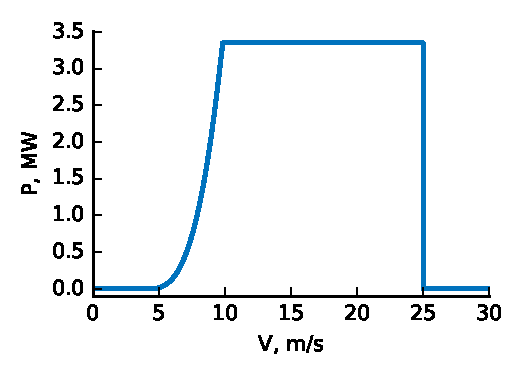
\includegraphics[]{./figures/power_curve.pdf}
	    \caption{Graphical depiction of IEA's 5-MW onshore reference turbine's power curve.}
	    \label{fig:5MW}
	\end{figure}
	%
	\begin{table}[H]
		\begin{center}
			\caption{Attributes for IEA's 5-MW onshore reference turbine}
			\label{tab:turb-att}
			\begin{tabular}{@{}lrl@{}}
			\toprule
				Rotor Diameter & 130 & m \\ 
				Turbine Rating & 5 & MW \\ 
				Cut-In Wind Speed & 4 & m/s \\ 
				Rated Wind Speed & 9.8 & m/s \\ 
				Cut-Out Wind Speed & 25 & m/s \\
			\bottomrule
			\end{tabular}
		\end{center}
	\end{table}
	
\subsubsection{Farm Geography}\label{sec:farmgeog}

	To focus on optimization method and EWM variability, as well as to avoid introducing too many unnecessary variables, the wind farms for all scenarios were on flat and level terrain.
%\subsubsubsection{Boundary Shape}
	To reduce boundary impacts on farm design, we chose a radially symmetric farm boundary.
	%Doing otherwise may have tended to give optimal turbine locations where turbines cluster at the farm corners or protrusions.
%\subsubsubsection{Turbine Placement}
	Turbine $(x, y)$ hub locations were restricted to be on or within the boundary radius.
	Turbines were further constrained to be no less than two rotor diameters apart from any other turbine.
%\subsubsubsection{Farm Diameter}

	Farm diameter sizing for each scenario needed to be restrictive enough to avoid simply placing all turbines on the boundary but also permit meaningful turbine movement by the optimizers.
	Although the participants were not required to use the example starting layouts that we provided, we tried to provide reasonable example layouts by dispersing the turbines as much as possible in an orderly way. This was done by placing turbines in evenly spaced concentric rings. The boundary radii of the various wind farms we defined were selected to permit turbine placement in concentric rings with a minimum turbine spacing of five rotor diameters.
	%The following algorithm was implemented to determine both farm boundary diameters and the example layouts (described in the next section) for all farms in the Studies:

    %\begin{enumerate}
    %    \item Place one turbine in the center of the farm
    %    \item Organize remaining turbines in concentric circles, maintaining a minimum of 5 diameter spacing both laterally and between rings
    %    \item If the outermost ring has less than 5 turbines:
    %    \begin{enumerate}
    %        \item Expand penultimate ring as little as possible to fit these outermost turbines, while maintaining the lateral spacing requirement
    %    \end{enumerate}
    %    \item Expand radius of outermost ring to the nearest $100$ m.
    %    \item Evenly expand the inner turbine rings for uniformity
    %\end{enumerate}

%\vspace{3mm}
%\noindent\textbf{Example Layouts}

%	\noindent These layouts are displayed below graphically in \cref{fig:exlayouts}. Though primarily for Case Study 1, they are provided to participants of both studies in \texttt{.yaml} format for 4 reasons:

%	\begin{enumerate}
%		\item To provide an example of the \texttt{.yaml} schema formatting being developed by IEA Task 37, used to enable collection of results
%		\item To help participants visualize the different farm sizes and geography
%		\item To verify AEP calculation if participants implement the Case Study 1 wake model in a different language
%		\item To provide participants with an optimization starting point if desired
%	\end{enumerate}

%	\begin{figure}[H]
%		\centering
%			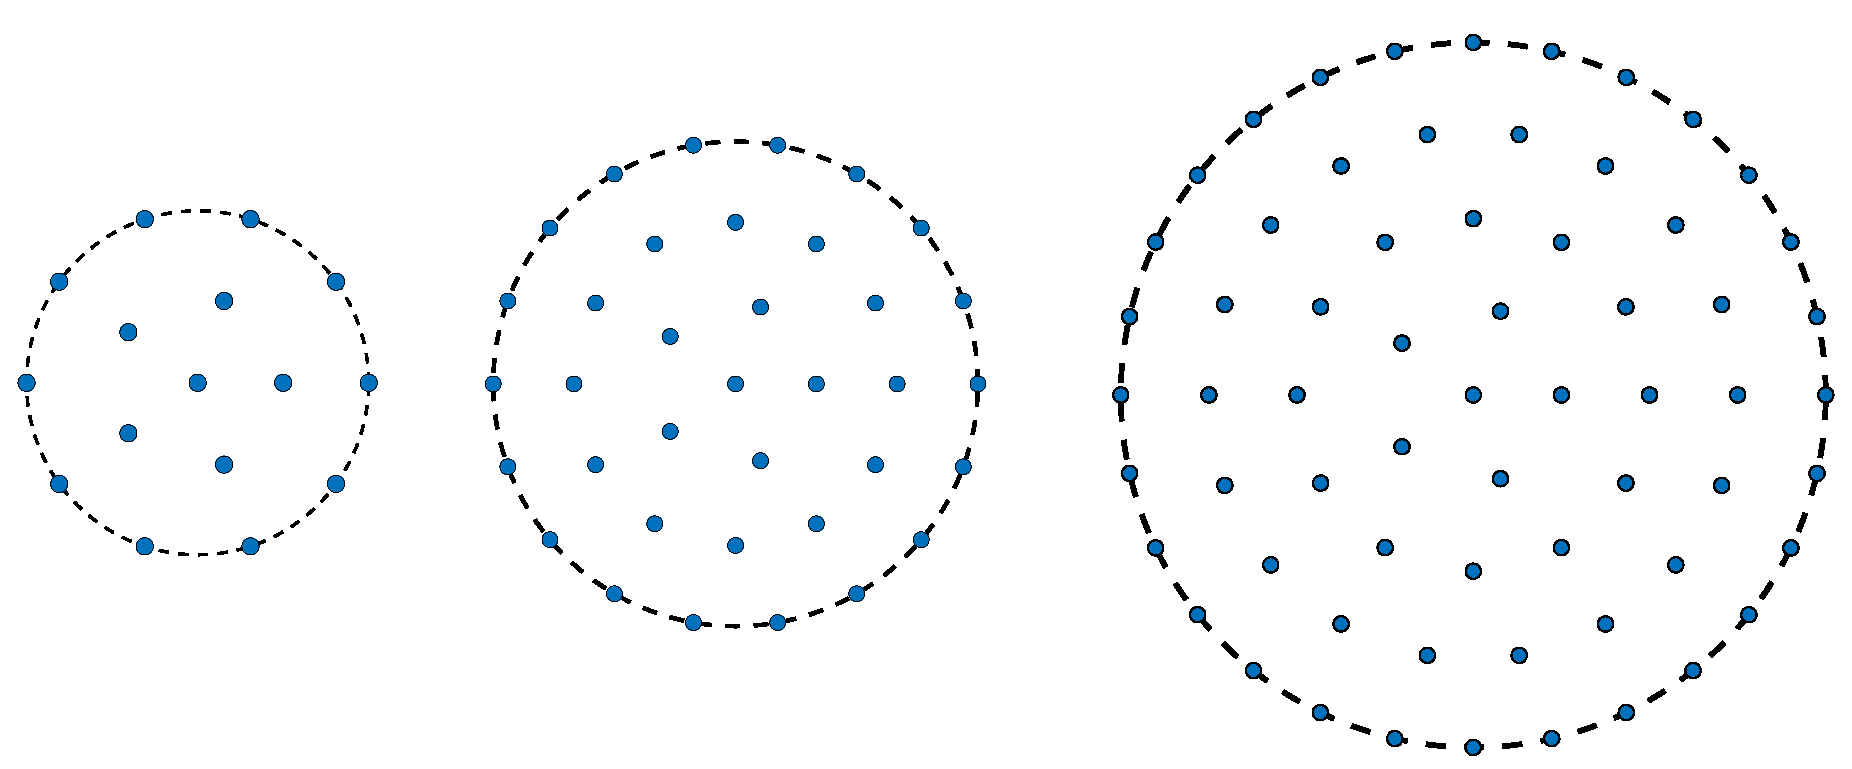
\includegraphics[width=\textwidth]{./figures/iea37-exfarms.pdf}
%		\caption{Example layouts for 16, 36, and 64 turbine farms}
%		\label{fig:exlayouts}
%	\end{figure}

%	It is explicitly stated in the announcement document that these layouts are only examples.
%	Participants are not required to use these as starting points for their optimizations, though they have the option to do so.

\subsubsection{Wind Attributes}

	The wind distribution frequency and wind speed were the same for all wind farm scenarios in both case studies.
%\subsubsubsection{Wind Speed}
	Freestream wind velocity was constant in all wind directions, at $9.8\ \textrm{m/s}$, regardless of turbine location or time of day.
	This wind speed was used because it is the rated wind speed of the IEA 3.35-MW wind turbine.
	Using this incoming wind velocity maximized power production variability between wind turbines in the farm.
	In setting the scenario's freestream velocity for the turbine's rated wind speed, any wake effects moved air speeds down below rated power.
	With greater variability in the power production, more local optima would be experienced by participant optimizers.
	%Conversely, if the incoming wind speed were placed higher than the rated wind speed (i.e. $13\ \textrm{m/s}$), more turbine layouts, though different in location, would produce identical power outputs, unaffected 
%\subsubsubsection{Wind Direction Frequency}
	%\noindent In creating these case studies, we desired a wind direction frequency distribution (displayed graphically in a wind rose) that meets two criteria:
	%\begin{enumerate}
	%	\item Creates many local optima
	%	\item Prevents dissimilar turbine layouts from reaching the same AEP values
	%\end{enumerate}
	A lack of such local optima in a design space permits even ineffective optimizers to find a superior result.
	%In a design space where local optima are present, inferior designs are very likely.
	Since the presence of many local optima is a feature observed on many wind farm optimization problems, we strove to create such design spaces with our case study scenarios,  as it allows us to test the exploration capabilities of the various optimization algorithms.
	
	The selection of the wind rose was a major factor in the frequency and magnitude of local optima resulting from turbine placement.
	%In our tests, uni-directional windroses often push turbines into a single row perpendicular to the major wind direction, hintng at a relative lack of local optima.
	%Omnidirectional roses that we tested tended towards a pattern of simply spreading the turbines out uniformly, also hinting at a lack of local optima.
	%We therefore intentionally designed a windrose with relatively many local optima, in order to demonstrate the difference in capabilities of the various optimization algorithms used by participants.
	%If, on the other hand, many unique layouts produce high and similar AEP values, it would likewise not tell us much regarding the abilities of participant optimization methods.
	%When many answers give superior results, algorithms are not incentivized to find one ``best'' result.
	%Therefore to acheive both of these criteria, we experimented with 4 different patterns of wind direction frequency:
	%\begin{enumerate}
	%	\item Bi-modal uniaxis (to simulate a canyon geography)
	%	\item Quad-directional (experienced at some onshore airports)
	%	\item Tri-direcitonal (experienced by some coastline geographies)
	%	\item Bi-modal off-axis (experienced in both on- and off-shore locations)
	%\end{enumerate}
	%Simulations were run using the simplified Gaussian wake model and the optimization package SNOPT.
	%We ran each wind rose through 1000 random-start optimizations.
	%All wind roses gave generally similar optimization results with AEP distributions following a bell-curve pattern.
	%There were slight differences, however, in that:
	%\begin{enumerate}
	%	\item Bi-modal uniaxis gave turbine arrangements that tended towards a straight line, perpendicular to the uniaxis of the wind. Since it met our first disqualifying criteria of a lack of local minima, it was not further analyzed.
	%	\item Quad-directional gave turbine arrangements that tended towards a grid pattern. Since this too didn't have many local optima to trap optimizers, it was disqualified.
	%	\item Tri-directional gave many gird-like arrangements that all had similar AEP values. Since it met our second disqualifying criteria of non-similar layouts producing similar AEP, it was not selected.
	%	\item Bi-modal off-axis gave few results with high AEP values. We interpreted this to be indicitive of the presence of many local optima. Since this best met our selection criteria, it is the wind rose utilized for our case studies.
	%\end{enumerate}
	We selected a wind rose with an off-axis wind frequency distribution, binned for 16 directions.
	When we tested this wind rose against 1,000 randomized starting turbine locations, it gave few optimized results with relatively high AEP values.
	We interpreted this to be indicative of the presence of many local optima.
    The wind rose we used is depicted in \cref{fig:freqdist}, in polar coordinates. In this figure, a greater magnitude in the radial direction from the origin indicates a higher wind frequency from that specific direction.
	
	\begin{figure}[H]
		\centering 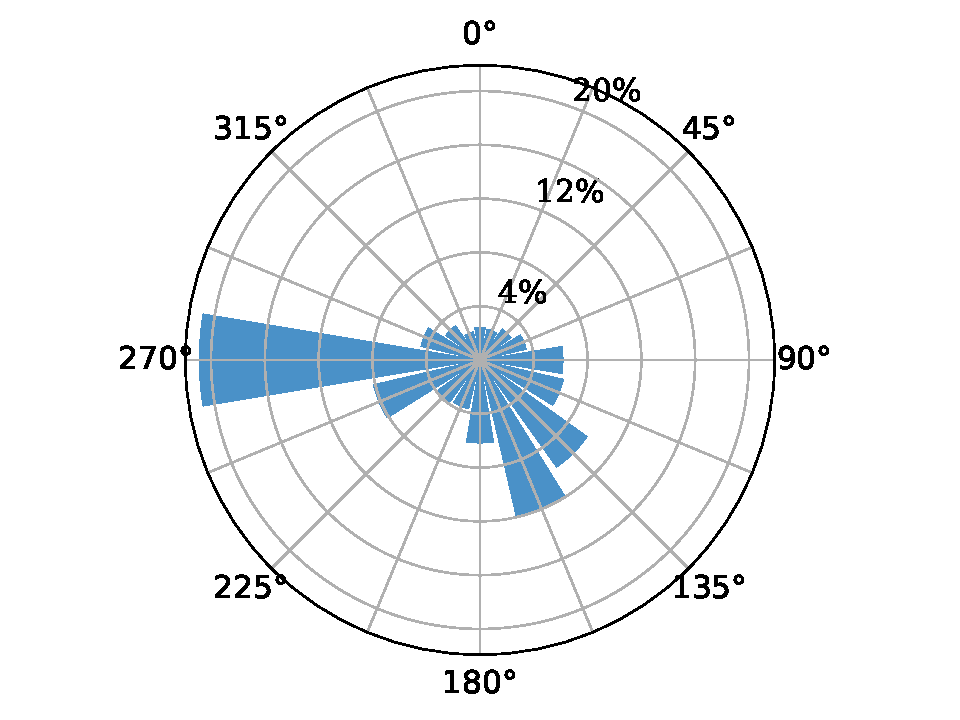
\includegraphics[width=.5\textwidth]{./figures/windrose.pdf}
		\caption{The wind frequency distribution for our case studies.}
		\label{fig:freqdist}
	\end{figure}

	%The quad-directional, tri-directional, and bi-modal off-axis roses are dipectied in \cref{fig:testroses}, and histograms of the 1000 random start optimizations are in \cref{fig:rosehists}.

	%\begin{figure}[H]
	%	\centering
	%		\caption{Quad-directional, Tri-directional, and Bi-modal off-axis wind roses}
	%		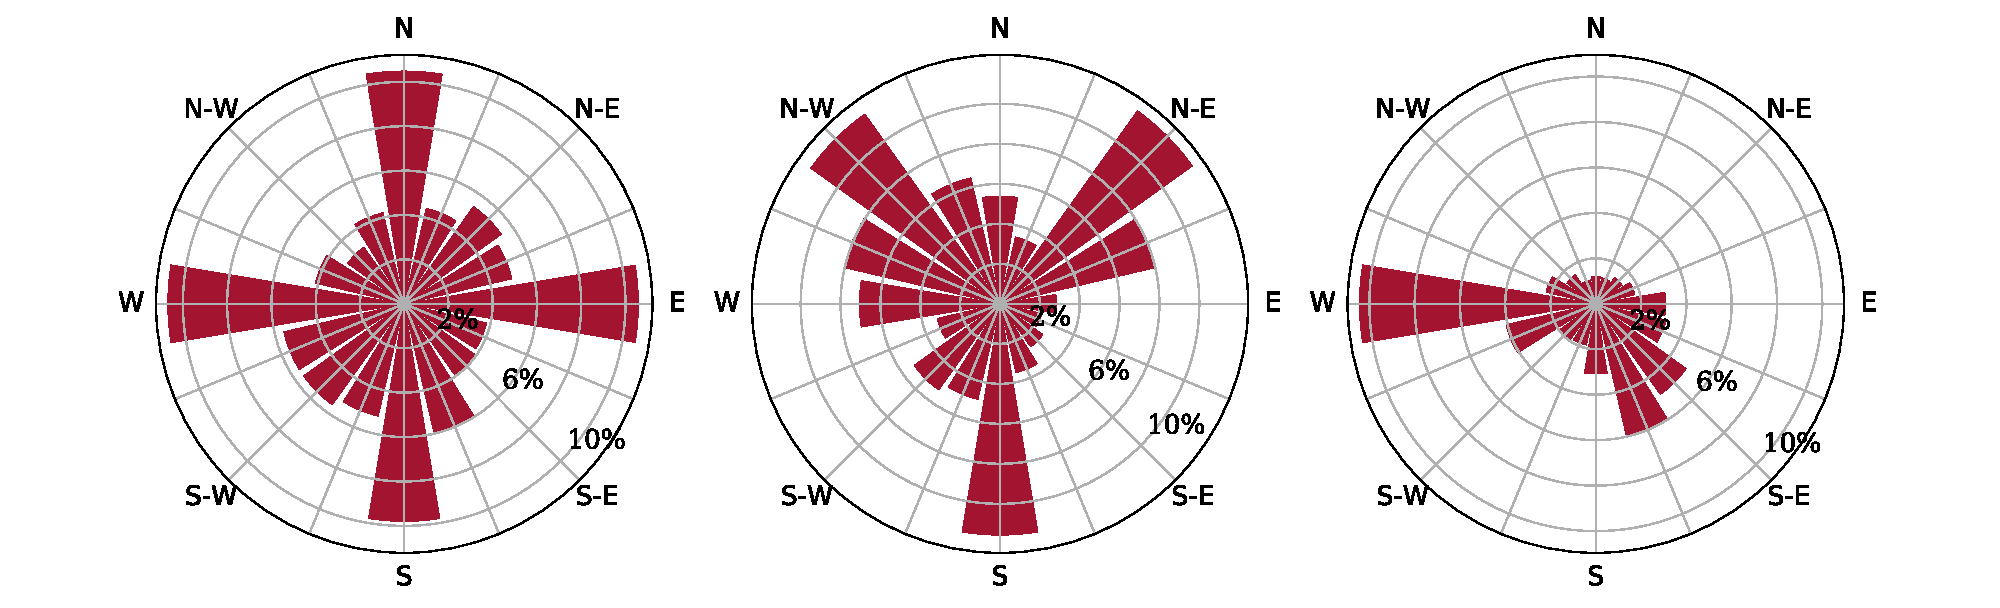
\includegraphics[width=\textwidth]{./figures/testroses.pdf}
	%	\label{fig:testroses}
	%\end{figure}

	%\begin{figure}[H]
	%	\centering
	%		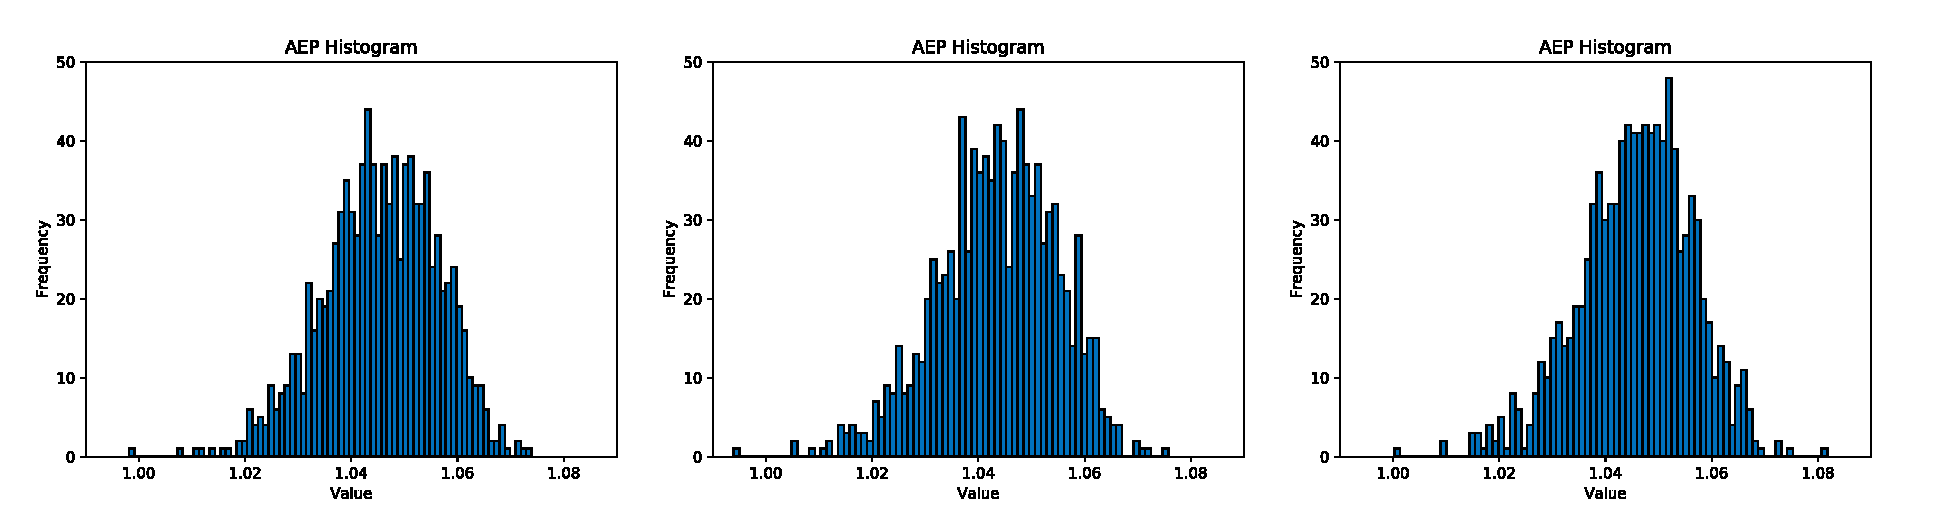
\includegraphics[width=\textwidth]{./figures/rosehists.pdf}
	%	\caption{1000 random start optimization runs for the Quad-, Tri-, and Bi-modal off-axis wind roses}
	%	\label{fig:rosehists}
	%\end{figure}

	%After the above described study, we selected the bi-modal off axis wind frequency distribution for our Case Studies, the rightmost windrose in \cref{fig:testroses}.

%\subsubsection{Data File Type} \label{sec:filetypes}
%	One request made by members of IEA Task 37 work package (WP) ten (X) was to implement the IEA 37 WP X's ontology open source \texttt{.yaml} schema for all necessary data.
%	This included:
%	\begin{itemize}
%		\item{Farm turbine attributes}
%		\item{Farm turbine locations}
%		\item{Farm wind frequency and wind speeds}
%	\end{itemize}

%	There exists a separate IEA37 working group tasked with refining the precise schema of these items, whose work is outside the scope of our specific Case Studies.
%	Though a current work in progress, we implemented the most recent iteration and adapted them to our scenarios as necessary.

%	The above mentioned data schema format is supplied to participants of both cases. They are:
%	\begin{enumerate}
%		\item \texttt{iea37-windrose.yaml} - binned wind frequency for both Case Studies, in \texttt{.yaml} format
%		\item \texttt{iea37-335mw.yaml} - data for reference turbine used in both Case Studies, in \texttt{.yaml} format
%	\end{enumerate}

%	Further examples for reporting turbine locations in \texttt{.yaml} schema, as well as a Python parser for all these schema was made available to Case Study participants.
%	Since the use of the example layouts and Python \texttt{.yaml} parser is more applicable to the Optimization Only Case Study, they are described in \cref{sec:optonly}.